% DDBM v2 -- calibrated rank test. Overleaf: pdfLaTeX + BibTeX.
% Needs references.bib and fig_mechanism.pdf alongside.
\documentclass[11pt]{article}

\usepackage[utf8]{inputenc}
\usepackage[T1]{fontenc}
\usepackage{lmodern}
\usepackage[margin=1in]{geometry}
\usepackage{amsmath,amssymb,amsthm}
\usepackage{booktabs}
\usepackage{graphicx}
\usepackage{microtype}
\usepackage{caption}
\usepackage{enumitem}
\usepackage[hidelinks,breaklinks]{hyperref}

\newtheorem{lemma}{Lemma}
\newtheorem{proposition}{Proposition}
\newcommand{\Xph}{\Xi}

\title{\bfseries Two Domain Errors in a Symbolic Test for\\
Deterministic Structure, and Their Repair:\\[4pt]
\large Exact Calibration, Surrogate Domain, and an Open Benchmark}

\author{Nazar Sotiriadi\thanks{\texttt{n.sotiriadi@gmail.com}}}

\date{Zenodo \href{https://doi.org/10.5281/zenodo.21924169}{10.5281/zenodo.21924169} (all versions:
\href{https://doi.org/10.5281/zenodo.18753232}{10.5281/zenodo.18753232}) --- supersedes version~1,
\href{https://doi.org/10.5281/zenodo.18753233}{10.5281/zenodo.18753233}\\[2pt]
\today}

\begin{document}
\maketitle

\begin{abstract}
\noindent
Version~1 of this work proposed DDBM, a screening test that quantizes a
rank-normalized scalar series onto an integer lattice, forms a modular phase
from a cubic kernel, and reads departures from uniformity as deterministic
structure. This version withdraws that detector claim and replaces it with a
procedure whose validity is established rather than assumed.

The organising finding is that a single principle governs both stages of such a
test, and that violating it in either place silently destroys validity:
\emph{every operation must be performed in the domain where its null is
defined}. Applied to the screening stage, this means the statistic may depend on
the data only through ranks; amplitude preprocessing performed beforehand
destroys distribution-freeness, driving empirical size at nominal $0.05$ to
$0.19$ on a lognormal marginal and $0.88$ on a Cauchy marginal, while
rank-only symbolization restores exactness with a one-line proof and gives
nominal size across six marginals. Applied to the confirmation stage, it means
IAAFT surrogates must be generated in normal scores --- the rank-based inverse
normal transform $\Phi^{-1}(\mathrm{rank}/(n+1))$, also called Gaussianization
--- which is the domain in which the AAFT null is stated. Generated from raw amplitudes they reject a static
monotone transform of an AR(1) process --- inside their own null --- in
\emph{every} replicate; generated from ranks they reject strongly autocorrelated
processes in $47\%$. In normal scores all three land on exactly the nominal $0.05$ over $100$
replicates, invariance under monotone transformation is restored, and power on
deterministic systems is unaffected. One failure survives the repair:
conditional heteroscedasticity, rejected at $0.15$, lies outside the IAAFT null
altogether and needs a model-based null.

We also report three secondary results. The cubic kernel is one member of a
cyclotomic family, with an exact identity for the phase lattice; the identity
appears to be new in this context but does not improve on simpler alternatives:
the phase is a lossy function of the pair $(N_t,\Delta N_t)$, and a classical
ordinal count needing neither modular arithmetic nor arbitrary-precision
integers is statistically indistinguishable from it while being far cheaper. The standard ordinal baseline is silently degenerate when every
pattern length in the grid is saturated, which at $n=10^4$ means $d\le 6$. And
S\&P~500 log returns, rejected by an IAAFT null, are not rejected by a fitted
GARCH(1,1) null: the apparent structure is conditional heteroscedasticity, so
the financial conclusion of v1 is not merely withdrawn but resolved.

No new detection principle is claimed --- the mechanism is the
forbidden/missing-pattern paradigm and coarse-grained transition statistics.
What is offered is a validated inference layer for those classical statistics,
a catalogue of the ways it fails, and a benchmark of 165 series whose 46 labeled
members are byte-reproducible and labeled by computed Lyapunov exponents. The
comparisons here are calibration on that set, not independent validation.
\end{abstract}

\section{What is withdrawn}

Version~1 claimed a new detector reaching $92.5\%$ accuracy ``without
phase-space reconstruction or training data''. Three claims do not survive.

\paragraph{Not embedding-free.} $\Xph_t$ is a function of the pair
$(N_t,N_{t+1})$: a two-dimensional delay vector with $m=2$, $\tau=1$, quantized
at resolution $1/K$. Scanning $K$ is a scan over box scale, and the count of
realized pairs is a single-scale box count in that embedding. The embedding
parameters were fixed and hidden, not eliminated.

\paragraph{The stated mechanism is self-cancelling.} v1 attributed the signal to
a singular marginal measure occupying few of $K$ cells. Rank normalization
removes exactly that: for a continuous marginal with $n\gg K$, every cell
receives about $n/K$ points however singular the underlying measure. What the
test sees is the geometry of transitions.

\paragraph{The $p$-values were invalid.} Phases from overlapping pairs are
serially dependent while the two-sample Kolmogorov--Smirnov test used to score
them assumes independence, and a Bonferroni correction over $K$ cannot repair a
miscalibrated individual test. Section~\ref{sec:screen} shows the defect runs
deeper: with the published order of operations the procedure is not even
distribution-free.

What is \emph{not} new is also worth stating. Discriminating determinism by the
occupancy of symbol transitions is classical: symbolic dynamics and forbidden
words~\cite{crutchfield}, the Bandt--Pompe symbolization~\cite{bandtpompe},
forbidden and missing ordinal patterns~\cite{amigo,zanin}, ordinal transition
networks~\cite{mccullough}, direct determinism tests~\cite{kaplanglass,sugihara}.
The confound of Section~\ref{sec:limits} --- smooth stochastic processes
imitating low-dimensional determinism --- dates
from~\cite{theiler1986,osborne}.

\section{One principle, two stages}

A test of this family has two stages, each with its own null, and each null
lives in a particular domain.

The \textbf{screening} stage asks whether the series is i.i.d. Its null is
invariant under every monotone reparametrization of the observable, so the
statistic must be a function of ranks alone. The \textbf{confirmation} stage
asks whether the structure exceeds a linear process. The AAFT/IAAFT null is
``a static monotone transform of a linear Gaussian process''
\cite{theiler1992,schreiber}, so the object whose spectrum must be matched is
the \emph{underlying Gaussian}, not the observed series.

Both requirements are elementary. Both were violated in v1 and in our own first
revision, in opposite directions, and in both cases the violation is invisible
without an explicit size study. Sections~\ref{sec:screen} and~\ref{sec:surr}
measure the damage and the repair.

\section{Stage one: the screening statistic must be a rank statistic}
\label{sec:screen}

\subsection{The defect}

The published pipeline applies OLS detrending, AR(1) prewhitening and
data-dependent volatility standardization to raw amplitudes, ranking only
afterwards. The ranks of the residual then depend on the unknown marginal.
Table~\ref{tab:pivot} measures the consequence: calibrate under a Gaussian null
with $B=1000$ replicates at $n=10^4$, then test i.i.d.\ draws from six
continuous marginals.

\begin{table}[h]
\centering
\caption{Empirical size at nominal $\alpha=0.05$ of the screening stage as
published, calibrated under a Gaussian null; $200$ series per cell. ``KS'' tests
the $p$-values against $U(0,1)$.}
\label{tab:pivot}
\begin{tabular}{lrrrr}
\toprule
marginal & size@.05 & size@.10 & KS & $p_{\mathrm{KS}}$ \\
\midrule
Gaussian      & 0.045 & 0.090 & 0.047 & 0.757 \\
uniform       & 0.045 & 0.080 & 0.081 & 0.134 \\
Student $t_3$ & 0.065 & 0.080 & 0.078 & 0.162 \\
lognormal     & \textbf{0.190} & 0.245 & 0.237 & $<0.001$ \\
exponential   & 0.065 & 0.110 & 0.107 & 0.018 \\
Cauchy        & \textbf{0.880} & 0.885 & 0.840 & $<0.001$ \\
\bottomrule
\end{tabular}
\end{table}

\noindent
At nominal $5\%$ the published test rejects i.i.d.\ Cauchy data $88\%$ of the
time. For a marginal without finite moments the fitted trend and AR(1)
coefficient are unstable, and that instability writes marginal-dependent
structure into the ranks of the residual.

\subsection{The repair}

\begin{proposition}[distribution-freeness]
\label{prop:pivot}
Let $x_1,\dots,x_n$ be i.i.d.\ from any continuous $F$, and let $T$ depend on
the sample only through the rank vector. Then the law of $T$ does not depend
on~$F$.
\end{proposition}

\begin{proof}
Continuity makes ties null, and the rank vector of an i.i.d.\ sample is uniform
on the $n!$ permutations for every continuous $F$; a statistic measurable with
respect to it has a law determined by $n$ alone.
\end{proof}

\noindent
The Monte-Carlo null is therefore exact only if every amplitude operation is
removed or performed after ranking. Table~\ref{tab:orders} compares four orders.

\begin{table}[h]
\centering
\caption{Worst deviation of empirical size from nominal $0.05$ across the six
marginals of Table~\ref{tab:pivot}. This is a separate, smaller run
($150$ series per cell, $B=400$), in which variant~A reproduces the defect at
$0.853$ rather than the $0.880$ of Table~\ref{tab:pivot}.}
\label{tab:orders}
\begin{tabular}{llr}
\toprule
variant & description & worst $|$size $-\,0.05|$ \\
\midrule
A & amplitude operations, then ranks (as published) & 0.803 \\
B & ranks, then the same amplitude operations & 0.043 \\
\textbf{C} & \textbf{ranks only, no amplitude operations} & \textbf{0.030} \\
D & ranks, then differencing & 0.030 \\
\bottomrule
\end{tabular}
\end{table}

\noindent
Only variant~C passes the uniformity test at every marginal, and it is the one
Proposition~\ref{prop:pivot} sanctions. Its cost is that trends and linear
autocorrelation are no longer removed before screening, so the confirmation
stage must carry that load alone. The preprocessing was in any case partly
redundant: removing linear structure is what the confirmation stage tests for.

\section{Stage two: surrogates must be generated in normal scores}
\label{sec:surr}

\subsection{The defect, and a diagnostic that identifies it}

A static monotone transform preserves ranks exactly. A rank statistic therefore
\emph{cannot} distinguish an AR(1) series from its cube, and any procedure that
does is broken. Table~\ref{tab:surr} shows that the procedure with amplitude-domain
surrogates does exactly that: it rejects AR(1) at the nominal rate and its cube
in every replicate.

\begin{table}[h]
\centering
\caption{Rejection rate of the confirmation stage at nominal $0.05$, by the
domain in which surrogates are generated. The first three processes are monotone
transforms of one another, so a correct procedure must give them the same rate.
Raw and normal-scores columns use $100$ replicates with Wilson $95\%$ intervals;
the rank column is a $30$-replicate run retained only to show the direction of
its failure. $B=49$ throughout. The last block gives the $p$-value on
deterministic systems, where rejection is desired, at $B=99$.}
\label{tab:surr}
\begin{tabular}{lccc}
\toprule
process & raw amplitudes & ranks ($30$) & \textbf{normal scores} \\
\midrule
AR(1), $\phi=0.9$   & 0.02 [0.01, 0.07] & 0.47 & \textbf{0.05} [0.02, 0.11] \\
cubed AR(1)         & \textbf{1.00} [0.96, 1.00] & 0.47 & \textbf{0.05} [0.02, 0.11] \\
exponentiated AR(1) & \textbf{1.00} [0.96, 1.00] & 0.47 & \textbf{0.05} [0.02, 0.11] \\
white Gaussian      & --- & 0.03 & 0.03 [0.01, 0.08] \\
sine ${+}$ noise    & --- & 0.03 & 0.00 [0.00, 0.04] \\
GARCH(1,1) returns  & --- & 0.10 & \textbf{0.15} [0.09, 0.23] \\
\midrule
logistic $r=4$      & 0.010 & 0.010 & 0.010 \\
H\'enon             & 0.010 & 0.010 & 0.010 \\
Lorenz $x$          & 0.010 & 0.010 & 0.010 \\
R\"ossler $x$       & 0.010 & 0.010 & 0.010 \\
Chua $x$            & 0.060 & 0.010 & 0.010 \\
\bottomrule
\end{tabular}
\end{table}

\noindent
The three monotone-transform rows agree only in the normal-scores column, where
all three sit at exactly the nominal $0.05$ with identical intervals. That
agreement is not a coincidence to be admired but the signature of a correctly
specified test, and its absence is a sufficient diagnostic of misspecification
--- one that costs three lines to run and that we recommend as routine.

One row is \emph{not} repaired. GARCH(1,1) returns are rejected at $0.15$
$[0.09,0.23]$ in normal scores, an interval excluding the nominal level: fixing
the domain fixes the monotone-transform failure but not conditional
heteroscedasticity, which lies outside the IAAFT null altogether and requires a
model-based null (\S\ref{sec:applied}). We note that a $30$-replicate version of
this table read $0.00$ for the same cell, an estimate the larger run overturns
--- the referees' insistence on replicate counts was well placed, and small size
studies should be treated with the same suspicion as small power studies.

A partial mechanism is visible in the spectral mismatch between data and
surrogate periodograms: for the cubed series it is $0.075$ in the raw domain
against $0.000$ in normal scores. But it is not the whole story, since the
exponentiated series has a raw-domain mismatch of only $0.002$ and is still
rejected always. The general reason is the one stated in Section~2: a static
nonlinearity changes the autocorrelation function, so matching the periodogram
of the transformed series targets the wrong object. This is the classical AAFT
bias~\cite{kugiumtzis,schreiber2000}, here quantified for transition statistics.

\subsection{The repair}

Map to normal scores, $\Phi^{-1}\!\big(\mathrm{rank}/(n+1)\big)$, generate IAAFT
surrogates there, and evaluate the rank statistic on them. Size returns to nominal on every process tested, monotone-transform invariance
is restored, and power on deterministic systems is preserved. Chua, which the
amplitude domain fails to reject at $p=0.060$, is rejected at $p=0.010$; with
$B=99$ this is a single case and we read it as evidence that power is not
reduced, not that it is improved.

\section{The recommended procedure}
\label{sec:proc}

\begin{enumerate}[leftmargin=*,nosep]
\item \textbf{Symbolize.} Rank-normalize to $[0,1]$, average ranks for ties. No
detrending, no prewhitening, no volatility scaling (\S\ref{sec:screen}).
\item \textbf{Screen.} Evaluate the statistic on a grid, standardize each cell
by a Monte-Carlo null, take the maximum, and report
$p=(1+\#\{T_{\text{null}}\ge T_{\text{obs}}\})/(1+B)$. Scan multiplicity is
inside the simulated null, so no Bonferroni correction is applied.
\item \textbf{Confirm.} If screening rejects, test against IAAFT surrogates
generated in normal scores (\S\ref{sec:surr}). For heteroscedastic data this is
not enough --- size reaches $0.15$ --- and a model-based null is required
(\S\ref{sec:applied}).
\item \textbf{Classify.} Confirmed structure that is extremely narrowband
(spectral concentration $>0.95$ or $|\mathrm{ACF}|>0.99$) is
\emph{(quasi-)periodic}; otherwise \emph{confirmed nonlinear}, split by
transition occupancy into \emph{compatible with low-dimensional determinism} and
\emph{nonlinear stochastic}. We avoid the label ``chaos'': no surrogate test
establishes determinism.
\end{enumerate}

\paragraph{Pattern length is not a free parameter, but a floor.} The expected
fraction of unobserved ordinal patterns under an i.i.d.\ null at $n=10^4$ is
$0.000$ for $d\le 6$, $0.138$ for $d=7$, $0.781$ for $d=8$ and $0.973$ for
$d=9$. A grid all of whose members are saturated yields a statistic that is
identically zero under the null, with vanishing variance and meaningless
standardized scores; an earlier draft of this paper used $d\in\{4,5,6\}$ at
$n=10^4$ and obtained an apparently excellent baseline from exactly that
degeneracy. Once at least one unsaturated length is present the choice is
immaterial: accuracy is $37/40$ for each of
$\{7\},\{8\},\{7,8\},\{6,7,8\},\{5,6,7,8\},\{7,8,9\}$ at nominal size.

\section{Benchmark and matched comparison}
\label{sec:bench}

\subsection{The benchmark}

165 series with recorded provenance; 46 carry labels. Synthetic labels are
computed: maps by direct variational iteration, flows by Benettin
renormalization on the ODE with the analytic Jacobian~\cite{benettin}, giving
$\lambda=0.900$ (Lorenz, $\rho=28$), $0.083$ (R\"ossler, $c=5.7$), $0.425$
(Chua), with negative values for the regular regimes. Stochastic and mixed cases
are labeled by construction, not by an exponent; ``detector-independent ground
truth'' would overstate this, and we do not use the phrase.

The labeled set and the byte-reproducible set coincide exactly: all 46 labeled
series are regenerated from fixed seeds and pinned by SHA-256 in the repository,
while the 119 unlabeled series come from live sources that grow over time
(Yahoo appends trading days; HadCET and the NOAA indices extend monthly) and are
therefore not reproducible. Everything that affects a reported score is frozen
and verifiable; everything that is not frozen is illustrative only.

Computing $\lambda$ corrected a label carried in v1, and the correction is
delicate. At $r=3.57$ the logistic map has $\lambda=0.01096$ with a bootstrap
interval $[0.0109,0.0111]$, so it is weakly chaotic, not ``Regular''. But
$r=3.57$ lies \emph{above} the accumulation point $r_\infty=3.5699457$ (where
$\lambda\approx2\times10^{-5}$), and $r=3.5705$ gives $\lambda=-0.0039$: the
parameter sits among periodic windows. We report it as correctly labeled and
hypersensitive; every statistic tested misses it.

The 46 series are not 46 independent systems --- several are coordinates of one
attractor or members of a parameter family --- so class-wise counts are reported
alongside totals.

\subsection{Comparison}

All statistics run through the identical procedure of Section~\ref{sec:proc}:
same calibration, same normal-scores confirmation, same decision rule, same
auxiliary criteria; only the discriminating statistic differs. Scoring is
strict, with the six chaos${+}$noise cases excluded rather than counted correct
under either label --- a v1 rule that inflated the apparent score by six
unloseable cases.

\begin{table}[h]
\centering
\caption{Matched comparison in the final configuration, 40 labeled series,
strict scoring. Size is the range of empirical screening size at nominal $0.05$
over the six marginals of Table~\ref{tab:pivot}.}
\label{tab:compare}
\begin{tabular}{lrl}
\toprule
statistic & accuracy & screening size range \\
\midrule
missing ordinal patterns, $d\in\{6,7,8\}$ & \textbf{37/40} & 0.067--0.100 \\
cyclotomic phase scan                     & 36/40 & 0.025--0.067 \\
pair occupancy $(N_t,\Delta N_t)$         & 34/40 & 0.033--0.092 \\
\bottomrule
\end{tabular}
\end{table}

\begin{table}[h]
\centering
\caption{Class-wise counts for the same runs. The phase statistic is the most
specific and the least sensitive; the occupancy statistic loses specificity on
strongly autocorrelated and non-stationary processes.}
\label{tab:classwise}
\begin{tabular}{lccc}
\toprule
& ordinal & phases & occupancy \\
\midrule
Chaos ($n=14$)   & 13/14 & 11/14 & 13/14 \\
Regular ($n=10$) & 9/10  & 9/10  & 9/10 \\
Noise ($n=16$)   & 15/16 & \textbf{16/16} & 12/16 \\
\bottomrule
\end{tabular}
\end{table}

\noindent
None of the three differences is statistically meaningful. Exact McNemar tests
on the paired outcomes give $p=1.00$ (ordinal vs.\ phases, $2$ vs.\ $1$
discordant), $p=0.25$ (ordinal vs.\ occupancy, $3$ vs.\ $0$) and $p=0.69$
(phases vs.\ occupancy, $4$ vs.\ $2$). On this benchmark the three statistics
are indistinguishable, and the case against the cyclotomic construction rests on
parsimony and on the majorization argument of Section~\ref{sec:cyclo}, not on
measured accuracy.

The classical baseline is nominally best in both surrogate configurations we
ran. The other two, however, \emph{exchange places}: with amplitude-domain surrogates
occupancy scored $35/40$ against $34/40$ for the phases, and with the corrected
normal-scores surrogates the order reverses to $36/40$ against $34/40$. A
ranking that flips when an unrelated stage is repaired is not a ranking; we
report it as direct evidence that accuracy at a single $\alpha$ on forty series
is too fragile to separate close competitors, and that the power curves listed
in Section~9 are not optional refinements.

The occupancy misses are diagnosable rather than mysterious. Random walk and
long-memory series violate the stationarity that IAAFT
assumes~\cite{schreiber2000}; and AR(1) at $\phi=0.9$ has a measured rejection
rate of $0.07$ (Table~\ref{tab:surr}), so a single realization rejecting is an
ordinary draw, not a defect --- which is the same fragility seen from the other
side.

These are calibration results on the set used to fix thresholds and select the
kernel, not an independent validation; a held-out family of generators remains
to be run.

\section{The cyclotomic identity, in brief}
\label{sec:cyclo}

With $S_p(N)=(N+1)^p-N^p$ the modulus is, by construction, a difference of
consecutive powers, and it factors into homogeneous cyclotomic polynomials
evaluated at two \emph{consecutive} integers,
\begin{equation}
S_p(N)=\prod_{d\mid p,\ d>1}\Phi_d(N+1,N),
\label{eq:cyclo}
\end{equation}
so that $\rho=(N+1)N^{-1}$ is an exact $p$-th root of unity modulo $S_p(N)$ and
the phase lattice has denominator $\Phi_n(1)$. Appendix~\ref{app:cyclo} gives
the statements, the one-line proofs and the numerical checks. Figure~\ref{fig:mech}
shows the resulting lattice: Lorenz under the cubic kernel concentrates at
$\{0,\frac13,\frac23\}$ as Eq.~\eqref{eq:cyclo} predicts, the tent map under the
quadratic kernel hits the exact resonance at $\frac12$, and a pseudorandom hash
applied to the same data preserves the number of occupied atoms while destroying
their arithmetic positions --- which is what isolates the arithmetic from the
mere counting.

\begin{figure}[t]
\centering
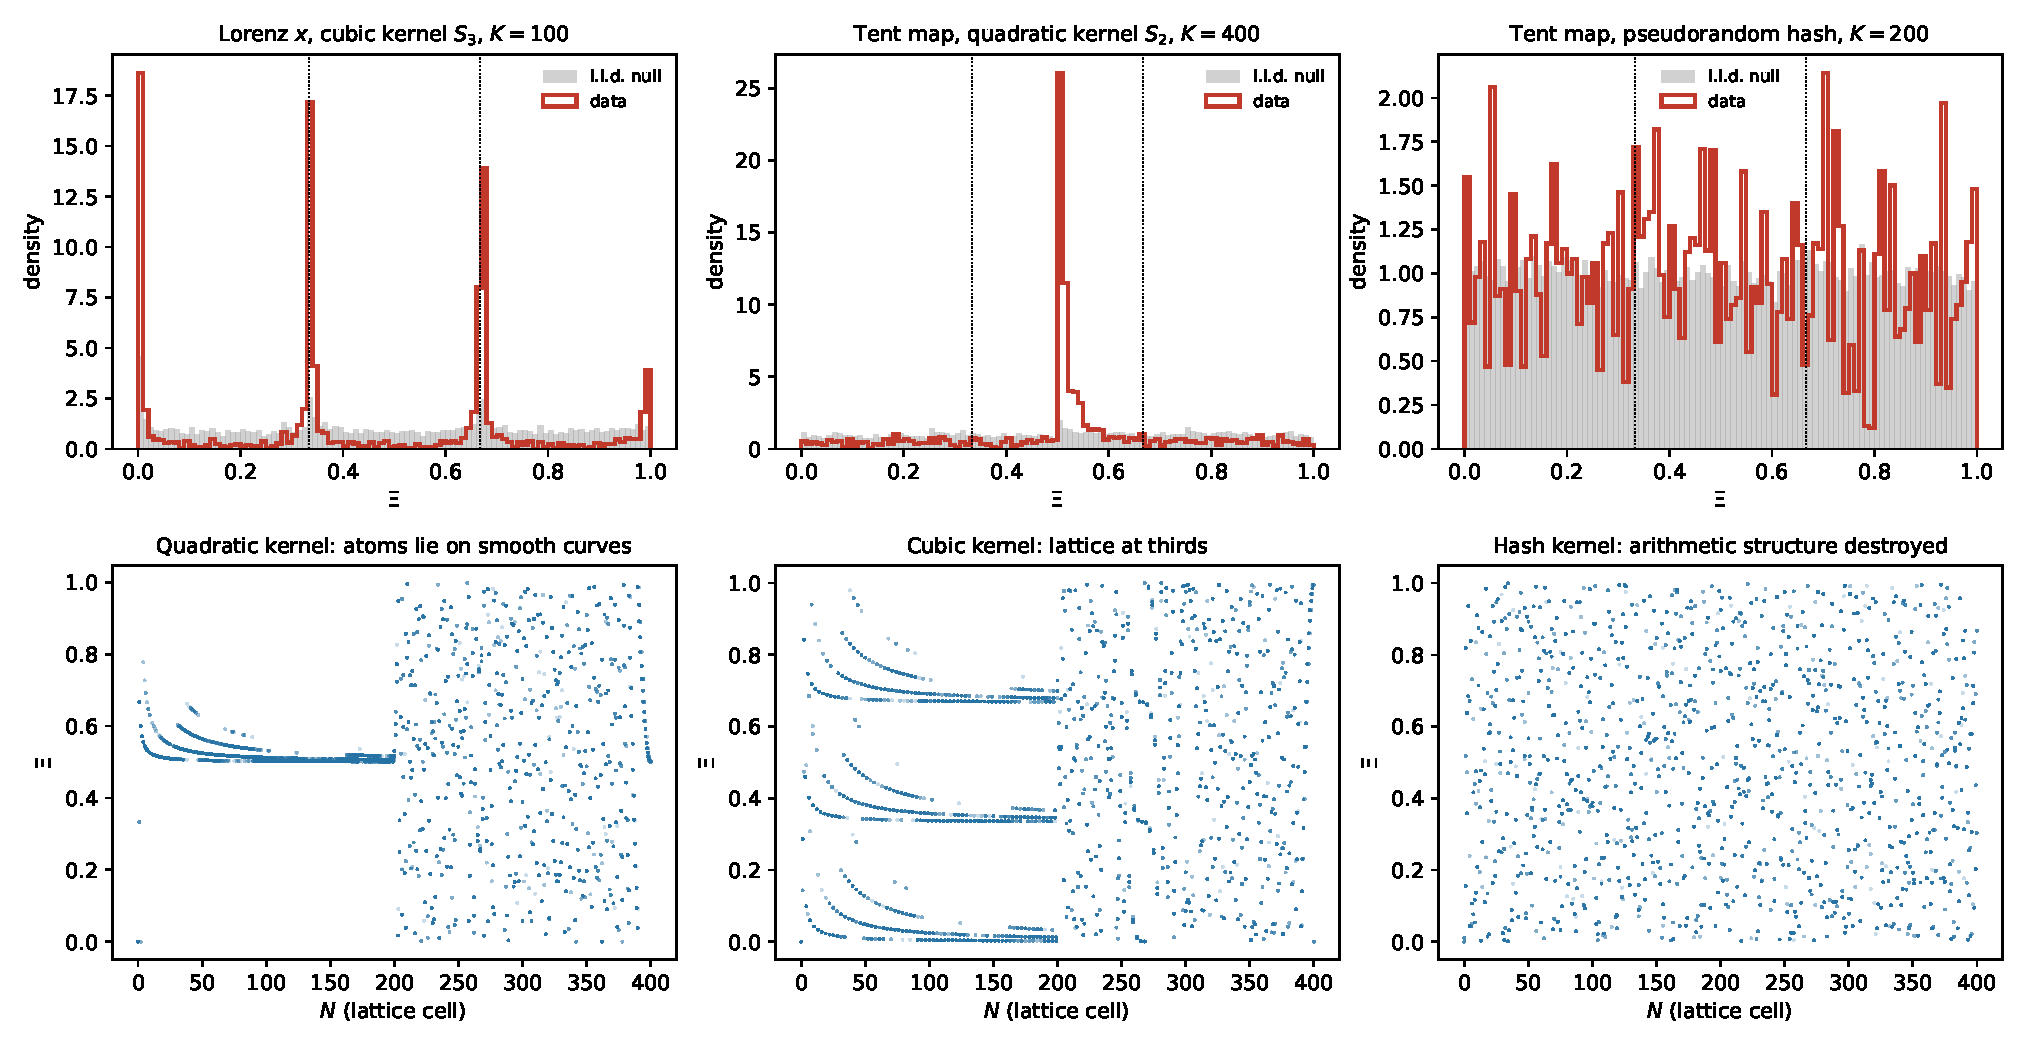
\includegraphics[width=\textwidth]{fig_mechanism.pdf}
\caption{Phase histograms against the i.i.d.\ null (top) and the atoms $\Xph$
against the lattice cell $N$ (bottom). The lattice predicted by
Eq.~\eqref{eq:cyclo} is visible in the first two columns and absent in the
third, where a hash replaces the polynomial kernel.}
\label{fig:mech}
\end{figure}

\paragraph{Why it does not help.} $\Xph$ is a deterministic function of
$(N_t,\Delta N_t)$, so any test on $\Xph$ is majorized by the \emph{best} test
on the pair: the phase map can only lose information. This is a statement about
the optimal test, not about our particular occupancy summary, and the empirical
comparison does not separate the three statistics
(Section~\ref{sec:bench}). What the comparison does establish is that a
classical ordinal count, requiring neither modular arithmetic nor
arbitrary-precision integers, is statistically indistinguishable from the phase
scan while being far cheaper --- which is sufficient reason not to prefer the
latter.

\section{Applied illustrations}
\label{sec:applied}

These are reported, not scored; ground truth is unavailable and their value is
agreement or disagreement with domain knowledge.

\paragraph{S\&P 500: resolved, not merely withdrawn.} The model-based null is a
parametric bootstrap: a GARCH(1,1) is fitted to the mean-centred series by
Gaussian quasi-maximum likelihood, $B=99$ independent paths of the same length
are simulated from the fitted model with Gaussian innovations, and the same
screening statistic is evaluated on each. Parameter estimation uncertainty is
\emph{not} propagated --- the null is conditional on $(\hat\omega,\hat\alpha,
\hat\beta)$ --- which makes the test mildly anti-conservative and therefore
conservative for our purpose, since we are accepting rather than rejecting this
null.

Under the corrected procedure, log returns over the full 1970--2026 history are
rejected by the IAAFT null ($p=0.02$) but \emph{not} by the fitted GARCH(1,1)
null ($p=0.31$;
$\hat\alpha=0.068$, $\hat\beta=0.924$). The 2010--2024 window behaves the same
way ($p_{\text{IAAFT}}=0.73$, $p_{\text{GARCH}}=0.33$). The apparent nonlinear
structure is conditional heteroscedasticity; there is no evidence of
low-dimensional determinism. Realized volatility is rejected by both nulls
($p=0.01$ each), which we report with the caveat that it is constructed by a
rolling window and is therefore smooth by design.

\paragraph{Climate.} Daily HadCET anomalies and monthly Ni\~no3.4, PDO and AMO
show no evidence of low-dimensional determinism within this test, consistent
with a stochastic climate model~\cite{hasselmann} and with the resolution of the
1980s attractor controversy~\cite{nicolis,grassbergerclimate}. Absence of
detection is not evidence of absence. Methodologically the important point is
that screening alone flags most of these series as structured, so a pipeline
without a confirmation stage would reproduce the error of that era.

\paragraph{EEG, with a confound.} On the Bonn data~\cite{andrzejak} the
confirmed-nonlinear rate rises monotonically across classes: $1/20$, $0/20$,
$1/20$, $4/20$, $17/20$ from healthy to ictal. Classes A/B are scalp recordings
and C/D/E intracranial, differing in modality and amplitude resolution, so the
gradient tracks that as well as clinical severity. No clinical claim is made.

\section{Limits}
\label{sec:limits}

\emph{Nonlinearity is not determinism.} GARCH volatility is nonlinear and
smooth (transition occupancy $0.41$, inside the deterministic range) and is
misclassified; a random walk sits at $0.17$. This is the effect
of~\cite{theiler1986,osborne} and a limit of surrogate methodology, not a
threshold to tune.

\emph{Instrumental quantization manufactures the signal.} RR intervals at
$128$\,Hz carry $50$--$79$ distinct values in $10^4$ points. Referencing the
occupancy statistic against a random permutation of the same values cancels the
value multiset exactly and largely removes the artifact ($0.04$--$0.09$ before,
$0.26$--$0.63$ after). A low-resolution flag accompanies every verdict, and we
decline to interpret the HRV results physiologically.

\emph{Densely sampled flows.} Most structure of a smooth oversampled flow lies
in the spectrum, so the confirmation stage has little power; reducing the flow
to successive local maxima repairs this on all six of our flows. The reduction
was devised on the cases that motivated it and is validated in-sample only.

\emph{Cost of dropping preprocessing.} Trends and linear autocorrelation now
reach the confirmation stage unfiltered, which costs power on strongly
autocorrelated linear processes.

\section{What is new, and what is not done}

\paragraph{New, as far as we can determine.} The identification of both domain
errors and their repair, with measured sizes before and after
(Tables~\ref{tab:pivot}--\ref{tab:surr}); the monotone-transform invariance
check as a cheap, sufficient diagnostic of surrogate misspecification; the
cyclotomic identification of the phase lattice, Eq.~\eqref{eq:cyclo} with
Lemma~\ref{lem:order}, correct and negative in consequence; the saturation floor
for ordinal pattern length; and a benchmark whose scored part is frozen and
labeled by computed exponents.

\paragraph{Not new.} The detection principle, the mathematics of cyclotomic
factorization and primitive divisors, the smooth-stochastic confound, and
surrogate methodology itself. The AAFT bias we quantify has been known
qualitatively since~\cite{kugiumtzis}.

\paragraph{Useful, and missing from current tooling.} Widely used packages
supply these statistics but not the inference around them:
\texttt{ordpy}~\cite{ordpy} computes permutation entropy, complexity--entropy
planes, missing patterns and ordinal networks, and provides no hypothesis test,
no $p$-values, no surrogate framework and no null calibration; surrogate
generators exist separately and are not wired to the statistics. The literature
itself notes that raw missing-pattern counts cannot be thresholded by
inspection~\cite{zanin}.

\section{Future work, in priority order}

\begin{enumerate}[leftmargin=*,nosep]
\item \textbf{Power curves over $n$ and SNR at fixed size.} Accuracy at a
single $\alpha$ on forty series cannot separate close competitors, as the
exchange of places in Section~\ref{sec:bench} and the McNemar tests both show.
Curves are the only way to rank these statistics honestly.
\item \textbf{Independent validation on held-out generators.} Thresholds, the
kernel and the decision rule were all fixed on the same 46 series, so
Table~\ref{tab:compare} is calibration. A frozen protocol applied to a family
of generators reserved in advance would make it validation.
\item \textbf{Model-based nulls for further classes.} The GARCH case of
Section~\ref{sec:applied} shows what a correctly specified null buys; the same
is needed for stochastic volatility, ARFIMA and non-stationary processes, for
which IAAFT is inappropriate by construction.
\item \textbf{Several realizations per system, with cluster-aware
uncertainty.} The benchmark contains coordinates of common attractors and
members of parameter families, so its 46 entries are not 46 independent draws.
\item \textbf{Out-of-sample validation of the return-map reduction}, which was
devised on the cases that motivated it.
\end{enumerate}

\section{Conclusion}

The construction proposed in v1 does not survive: it is a lossy projection of a
pair statistic that itself rediscovers a classical mechanism, and at matched
nominal size it is the weakest statistic we compared. Its cubic kernel has an
exact cyclotomic explanation, which is satisfying and useless.

What survives is a principle and its consequences. Each stage of a symbolic test
must be carried out in the domain where its null is defined: rank-only
symbolization for screening, normal scores for surrogate generation. Both
requirements are elementary, both were violated here in opposite directions, and
neither violation is visible without an explicit size study --- one drove
empirical size to $0.88$, the other to $1.00$. Together with a monotone-transform
invariance check that detects the second failure in three lines, and a benchmark
whose scored part is frozen and independently labeled, that makes a usable
procedure with stated limits. It is less than v1 claimed and more than it
delivered.

\section*{Reproducibility}

Code, benchmark manifest, checksums and result tables are in the \texttt{v2}
branch of \url{https://github.com/Theclimateguy/DDBM/tree/v2}.
\texttt{build\_dataset.py} regenerates or downloads all series and
\texttt{hash\_manifest.py} verifies them; \texttt{pivotality\_fix.py} reproduces
Table~\ref{tab:orders}; \texttt{reviewer\_experiments.py} Table~\ref{tab:pivot}
and the Lyapunov intervals; \texttt{surrogate\_domain.py} and
\texttt{surrogate\_normalscores.py} Table~\ref{tab:surr};
\texttt{essential\_revisions.py} the pattern-length study and the S\&P case;
\texttt{final\_benchmark.py} Table~\ref{tab:compare};
\texttt{cyclotomic\_kernels.py} the symbolic derivations of
Appendix~\ref{app:cyclo}; \texttt{size\_study\_100.py} the $100$-replicate size
study. Seeds are fixed throughout. Results here were produced with Python
3.13.11, NumPy 2.4.2, SciPy 1.17.1, SymPy 1.14.0 and Matplotlib 3.10.8.

\section*{Acknowledgements}

Three independent referee reports on the v1 and draft-v2 manuscripts identified
the embedding claim, the pivotality gap, the unvalidated confirmation stage, the
scoring rule, the baseline specification and the benchmark's reproducibility
status. Sections~\ref{sec:screen}--\ref{sec:surr} and the S\&P case study exist
because of them.


\appendix

\section{The cyclotomic identity in full}
\label{app:cyclo}

With $S_p(N)=(N+1)^p-N^p$ we have $(N+1)^p\equiv N^p \pmod{S_p(N)}$ by
construction.

\begin{lemma}
\label{lem:order}
For $N\ge1$ and $p\ge2$, $\gcd(N,S_p(N))=1$ and
$\rho=(N+1)N^{-1}\bmod S_p(N)$ has multiplicative order exactly $p$.
\end{lemma}

\begin{proof}
$S_p(N)=\sum_{j<p}\binom{p}{j}N^{j}\equiv1\pmod N$, so $N$ is invertible, and
$\rho^{\,p}\equiv1$ makes the order divide $p$. Were it $d<p$ with $d\mid p$,
$S_p(N)$ would divide $(N+1)^d-N^d$, a positive integer strictly smaller than
$S_p(N)$ for $N\ge1$ --- impossible.
\end{proof}

\noindent
The cell $N=0$ must be excluded: $S_p(0)=1$, the ring is trivial and $N^{-1}$
does not exist. Expanding the difference of powers gives Eq.~\eqref{eq:cyclo},
$S_p(N)=\sum_{j=0}^{p-1}(N+1)^{j}N^{\,p-1-j}=\prod_{d\mid p,\ d>1}\Phi_d(N+1,N)$,
verified symbolically for $p=2,\dots,6$. Since the arguments are coprime the
Bang--Zsigmondy primitive-divisor theory~\cite{zsigmondy} applies: every prime
divisor $q$ of $\Phi_p(a,b)$ satisfies $q\equiv1\pmod p$ except possibly $q=p$
(no violations for $p\in\{3,5,7\}$, $N\in[2,200]$). Hence $p$ divides
$|(\mathbb{Z}/S_p)^\times|$ and an element of order $p$ must exist.

For $p=3$, $3N^3=S_3(N)(N-1)+(2N+1)$ places the phases at
$\Xph(N,0)=k/3+O(1/N)$; the median distance to $\{0,\frac13,\frac23\}$ is
$2.2\times10^{-4}$ over $N\in[2,2000]$. In general the lattice denominator is
$\Phi_n(1)$, which is $p$ for $n=p^k$ and $1$ otherwise, matching measurement
for $n=2,\dots,12$. This is proved for $\Delta N=0$ and for the tent-map branch
where $\Delta N=N$ gives the exact resonance
$\Xph=(N{+}1)/(2N{+}1)\to\frac12$; that an arbitrary deterministic trajectory
concentrates on the lattice more than a stochastic one is an empirical
observation, not a theorem.

\bibliographystyle{unsrt}
\bibliography{references}

\end{document}
